% TestVDB — VLDB draft (acmart sigconf, anonymous review, 2026-07-10)
% Compile: pdflatex paper-draft-vldb; bibtex paper-draft-vldb; pdflatex x2

\documentclass[sigconf, anonymous, review]{acmart}

\setcopyright{none}
\acmConference[]{}{}{}

\usepackage{booktabs}
\usepackage{graphicx}
\usepackage{amsmath}
\usepackage{listings}
\usepackage{xcolor}
\usepackage{enumitem}
\usepackage{tikz}
\usetikzlibrary{positioning, arrows.meta, calc}

\lstdefinestyle{curl}{
  basicstyle=\ttfamily\scriptsize,
  breaklines=true,
  keywordstyle=\color{blue},
  stringstyle=\color{teal},
  frame=single,
}

\ccsdesc[500]{Software and its engineering~--~Software testing and debugging}
\ccsdesc[300]{Information systems~--~Specialized database management systems}

\keywords{Vector database, API compliance defects, LLM-driven testing, test oracle, contract hallucination, multi-agent verification}

\title{TestVDB: Detecting API Compliance Defects in Vector Database Systems via Contract-Truth Separation}
\author{Anonymous Author(s)}
\affiliation{\institution{Anonymized for review}}

\begin{document}

\begin{abstract}
Vector Database Management Systems (VDBMSs) have become critical infrastructure for Large Language Model (LLM) applications, yet their reliability is underexplored: incorrect-behavior defects account for 43\% of VDBMS bugs---far exceeding crash/hang bugs (23\%)---and current fuzzers such as VDBFuzz rely on crash oracles that cannot detect this majority class. We introduce \emph{API compliance defects}---bugs where a VDBMS silently accepts inputs or produces behaviors that violate its documented contract---as a tractable, previously unsystematized slice of this gap, and present \textbf{TestVDB}, the first LLM-driven detector for them. TestVDB auto-derives a contract oracle from official API documentation and applies \textbf{Contract-Truth Separation} (CTS): it isolates LLM-generated assertions from a truth layer that falsifies them through maintainer-authority evidence (source grounding, clean reproduction, by-design intent). CTS is necessary because we identify and characterize \emph{contract hallucination propagation}: when an LLM both generates a contract and judges compliance, hallucinated constraints are self-confirmed in the generation--judgment chain---12 of our submissions were judged by maintainers as by-design---the LLM-derived contract was stricter than the true intent. Across five VDBMSs, TestVDB produced 111 candidate issues; maintainers acknowledged 36 (28 fixed, 8 accepted), raising end-to-end precision to 69.2\% across five VDBMSs (36 of 52 maintainer-adjudicated issues); a controlled retrospective further shows the dev-reviewer's source anchor lifts false-positive suppression from 31\% to 81\%. We state the system's boundary honestly: it specializes in boundary/validation compliance (75\% of yield), is complementary to crash-focused fuzzing, and does not solve the result-correctness oracle (ANN recall, ranking), which remains open.
\end{abstract}

\maketitle

%=========================================================================
\section{Introduction}\label{sec:intro}

VDBMSs such as Milvus, Qdrant, Weaviate, Chroma, and MeiliSearch now underpin retrieval-augmented generation, recommendation, and multimodal search. As they enter production at scale, their reliability directly affects downstream decisions. A study of 1{,}671 bug-fix pull requests across 15 VDBMSs~\cite{bugstudy25} finds that more than half of all defects are functional failures; a complementary testing roadmap~\cite{roadmap25} reports that \emph{incorrect-behavior} bugs (43.0\%) substantially outnumber crash/hang bugs (23.1\%).

Despite this distribution, current VDBMS testing skews toward the minority. VDBFuzz~\cite{vdbfuzz26}, the first dedicated VDBMS fuzzer, uses crash as its oracle and detects only crash/hang bugs, leaving the majority without a practical oracle. The roadmap~\cite{roadmap25} flags this as the central open challenge: incorrect behavior ``poses significant challenges for test oracles,'' and approximate vector search renders traditional differential testing unsuitable. Its Future Work asks both for ``an oracle for evaluating the correctness of vector search results'' and for methods that let LLMs ``stay updated with the latest syntax and functionalities.''

We target a tractable slice of this gap: \emph{API compliance defects}---bugs where the VDBMS silently accepts an input or produces a behavior that violates its documented contract (e.g., accepting \texttt{nprobe=0}, silently normalizing \texttt{shardsNum=-1}, or returning success where the docs prescribe rejection). These bugs do not crash, but they corrupt query semantics, lower recall, and expand the attack surface. Crucially, they admit an oracle where general result-correctness does not: the API contract itself.

\paragraph{Why an LLM, and why that is not enough.}
Compliance defects produce no observable failure signal, and VDBMS APIs have no widely-agreed reference implementation for differential testing. By exclusion (Table~\ref{tab:exclusion}), the only candidate oracle capable of flexible semantic judgment over an undocumented boundary is an LLM. But using an LLM as the oracle introduces two unreliable roles: it \emph{generates} the contract (from docs) and it \emph{judges} compliance---and both can hallucinate.

\begin{table}[t]
\caption{Oracle candidates for API compliance defects.}
\label{tab:exclusion}
\small
\begin{tabular}{@{}p{0.32\columnwidth}p{0.58\columnwidth}@{}}
\toprule
Candidate oracle & Why it fails for compliance defects \\
\midrule
Crash (VDBFuzz~\cite{vdbfuzz26}) & Compliance defects do not crash \\
PoC reproduction & No observable failure signal \\
Differential testing & No reference implementation for VDBMS APIs \\
Equivalence transformation & No query form to transform equivalently \\
\textbf{LLM} & \textbf{Only flexible semantic candidate---but it both generates the contract and judges, both unreliable} \\
\bottomrule
\end{tabular}
\end{table}

\paragraph{Core reversal: the oracle itself may be wrong.}
The naive design---an LLM extracts a contract from docs, then the same family of models judges compliance against it---is brittle because of \emph{contract hallucination propagation}. We observed a concrete instance: the formalizer ``extracted'' a complexity requirement from \texttt{constant.go} that is in fact a guard against a historical performance regression, not a behavioral constraint; the judge then confirmed violations against it. Across our submissions, 12 were marked by-design (\S\ref{sec:hallucination}): the LLM-derived contract was stricter than the maintainers' intent (demanding rejection of idempotent duplicate creates, eventual-consistency staleness, or lenient defaults). When the same model family generates the contract and judges compliance, hallucinated constraints are self-confirmed.

\paragraph{Approach: Contract-Truth Separation.}
When no mechanical oracle is available, the only usable truth source is \emph{maintainer authority}---source code, prior PRs, by-design intent, issue history. It is scarce, so it must be proxied by an agent. We separate the \emph{assertion layer} (LLM-generated contracts and judgments) from a \emph{truth layer} and use the latter to falsify the former. The truth layer is a dev-reviewer agent that applies counter-evidence along three anchors: clean reproduction, source-grounded verification (the direct counter to hallucination), and threat-model cross-check. This mirrors how a maintainer adjudicates an incoming bug report.

\paragraph{Results.}
TestVDB produced 111 candidate issues across five VDBMSs; maintainers acknowledged 36 (28 fixed, 8 accepted-open). The dev-reviewer removes 79\% of false positives (26/33) on a Milvus ablation batch, and end-to-end precision reaches 69.2\% (36/52) across five VDBMSs; a controlled retrospective shows its source anchor lifts false-positive suppression from 31\% to 81\%. We report the boundary honestly: 75\% of yield is boundary/validation compliance; crash bugs are excluded by design (complementary to VDBFuzz); soft result-correctness (approximate nearest neighbor (ANN) recall, ranking) remains open.

\paragraph{Positioning.}
We respond to VDBFuzz's generation-side Future Work (LLM-generated diverse API interactions and staying current with evolving APIs). Our judgment side provides a contract oracle that extends detection beyond crash into the API-compliance subset of incorrect behavior. We do \emph{not} claim to solve VDBFuzz's oracle-for-correctness direction (result correctness of vector search), which remains open~\cite{roadmap25}.

\paragraph{Contributions.}
\begin{enumerate}[leftmargin=*,itemsep=2pt]
\item The \textbf{first LLM-driven realization and large-scale empirical study of VDBMS API-compliance defect detection}---on the agenda defined by~\cite{roadmap25}, the first end-to-end realization for non-crash compliance defects, validated at scale (111 issues, 36 acknowledged).
\item \textbf{Contract-Truth Separation and its counter-evidence mechanism}: a design principle isolating LLM-generated assertions from a maintainer-authority truth layer (the dev-reviewer, three anchors) that falsifies them---removing 79\% of FPs (26/33) on a Milvus ablation; on a controlled retrospective its source anchor lifts FP suppression from 31\% to 81\% with TP recall $96.7\%$ ($n{=}30$, independent blind judge).
\item The \textbf{contract hallucination propagation finding}: when an LLM both generates a contract and judges compliance, hallucinated constraints are self-confirmed---observed in 12 by-design cases; the dev-reviewer's counter-evidence anchors are the mitigation.
\item \textbf{Empirical results and an open-source system}: 111 issues across 5 VDBMSs, 36 maintainer acknowledgments; an anonymized artifact is available at \url{https://anonymous.4open.science/r/testvdb-anon-D644/}.
\end{enumerate}

%=========================================================================
\section{Background and Problem Formulation}\label{sec:bg}

\subsection{VDBMS Architecture}
A VDBMS stores, indexes, and queries dense vector embeddings across a storage engine, a vector index (HNSW, IVF, etc.), a query processor (search, filtered/predicated search, multi-vector search), and client SDKs exposing REST and gRPC APIs~\cite{roadmap25}. Our targets live at the API surface and the query-processing logic behind it.

\subsection{Bug Taxonomy and Our Scope}
We adopt the symptom-level taxonomy of~\cite{roadmap25} as our primary frame (Crash/Hang 23.1\%, Incorrect Behavior 43.0\%, Performance 9.3\%, Build 9.7\%) and corroborate it with the larger empirical study~\cite{bugstudy25} (5 symptom categories, 31 fault patterns) used as a fault-pattern vocabulary. Our compliance-dimension axis projects onto the symptom axis as in Table~\ref{tab:scope}: we operate inside Incorrect Behavior, specialize in its boundary/validation subset, and exclude Crash (by design), Performance, and Build.

\begin{table}[t]
\caption{TestVDB scope projected onto the roadmap symptom taxonomy~\cite{roadmap25}.}
\label{tab:scope}
\small
\begin{tabular}{@{}p{0.42\columnwidth}p{0.48\columnwidth}@{}}
\toprule
Symptom class (share) & TestVDB coverage \\
\midrule
Crash/Hang (23.1\%) & Out of scope (L1 gate filters; 1 incidental in yield) \\
Incorrect Behavior (43.0\%) & \textbf{In scope}: boundary/validation (75\% of yield) + diagnostic + state/logic subsets \\
Performance (9.3\%) & Out of scope \\
Build (9.7\%) & Out of scope \\
\bottomrule
\end{tabular}
\end{table}

\subsection{API Compliance Defects}
An \emph{API compliance defect} is a behavior where, for an input governed by a documented or implementable contract, the VDBMS (i) accepts an input the contract prescribes to reject (\emph{illegal success}), (ii) rejects or mishandles an input the contract prescribes to accept, or (iii) returns a response whose status, payload, or side effects violate the contract (\emph{poor diagnostics / state violation}). The contract is not assumed perfect; Section~\ref{sec:hallucination} confronts contract unreliability directly.

\subsection{The Oracle Problem}
Compliance defects produce no crash and no exception, and---unlike SQL---there are no widely-agreed reference semantics for VDBMS APIs across vendors. Differential testing is unsuitable because APIs diverge and results are approximate~\cite{roadmap25}. Metamorphic relations~\cite{metmap24} serve result correctness but not API-acceptance decisions. The contract itself is the only candidate oracle---but it must be obtained and trusted, which is the core problem we address.

%=========================================================================
\section{Approach}\label{sec:approach}

\subsection{Overview}
TestVDB is a five-stage pipeline (Figure~\ref{fig:overview}): (1) contract extraction from API documentation via an LLM knowledge-extractor; (2) attack generation by specialized agents guided by a threat-model prior; (3) a four-judge debate producing Stage-2 candidates; (4) a dev-reviewer that applies Contract-Truth Separation as counter-evidence; (5) a two-layer novelty gate. A threat-model artifact is reused across stages as an experience prior.

\begin{figure}[t]
\centering
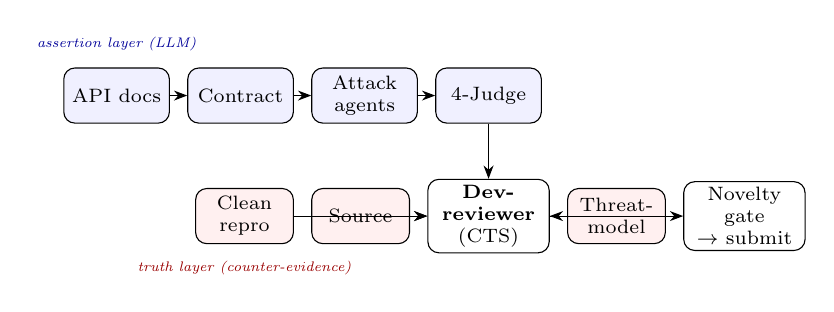
\begin{tikzpicture}[
  node distance=2.2mm and 2.2mm,
  font=\scriptsize,
  assert/.style={draw, rounded corners, fill=blue!6, align=center, inner sep=2pt, text width=12mm, minimum height=7mm},
  truth/.style={draw, rounded corners, fill=red!6, align=center, inner sep=2pt, text width=11mm, minimum height=7mm},
  gate/.style={draw, rounded corners, align=center, inner sep=2pt, text width=14mm, minimum height=7mm},
  arr/.style={-Stealth, thin}
]
\node[assert] (docs) {API docs};
\node[assert, right=of docs] (contract) {Contract};
\node[assert, right=of contract] (attack) {Attack\\agents};
\node[assert, right=of attack] (judge) {4-Judge};
\node[gate, below=7mm of judge] (devrev) {\textbf{Dev-reviewer}\\\scriptsize(CTS)};
\node[truth, left=of devrev] (src) {Source};
\node[truth, left=of src] (repro) {Clean\\repro};
\node[truth, right=of devrev] (tm) {Threat-\\model};
\node[gate, right=of tm] (out) {Novelty gate\\$\to$ submit};
\draw[arr] (docs)--(contract);
\draw[arr] (contract)--(attack);
\draw[arr] (attack)--(judge);
\draw[arr] (judge)--(devrev);
\draw[arr] (repro)--(devrev);
\draw[arr] (src)--(devrev);
\draw[arr] (tm)--(devrev);
\draw[arr] (devrev)--(out);
\node[font=\tiny\itshape, color=blue!60!black] at ($(docs.north)+(0,3mm)$) {assertion layer (LLM)};
\node[font=\tiny\itshape, color=red!60!black] at ($(repro.south)+(0,-3mm)$) {truth layer (counter-evidence)};
\end{tikzpicture}
\caption{TestVDB pipeline. The assertion layer (LLM contract + 4-judge) is falsified by the dev-reviewer's three counter-evidence anchors (truth layer). CTS = Contract-Truth Separation.}
\label{fig:overview}
\end{figure}

\subsection{Contract Extraction and the Threat-Model Prior}\label{sec:tm}
A knowledge-extractor agent crawls official API documentation and emits structured contracts (parameter domains, enum values, documented limits, status-code semantics) that seed both attack agents and judges. A threat-model artifact encodes recurring by-design intents (idempotency, eventual consistency, lenient defaults) and known blind spots; it is injected as a prior at generation (steering attacks toward non-trivial boundaries), at judgment (as a counter-evidence dictionary for the dev-reviewer), and at dedup. We treat the threat model as an \emph{exploratory pilot} (Section~\ref{sec:eval-tm}) rather than a core claim, because our ablation could not cleanly isolate its effect.

\subsection{Attack Generation and the Four-Judge Debate}
Three attack agents target the compliance dimensions: a \emph{boundary} agent (illegal-success at parameter, enum, and limit edges---the dominant yield), a \emph{semantic} agent (diagnostic-quality violations), and a \emph{state} agent (state/logic inconsistencies). Candidates enter a four-judge debate (evidence/severity/novelty/doc axes) drawing on multi-agent verification ideas~\cite{du2023improving}. The Stage-2 output of this debate feeds the dev-reviewer.

\subsection{Contract-Truth Separation and the Dev-Reviewer}\label{sec:cts}
Single-layer LLM judgment is unreliable because the same model family generates the contract and judges compliance. CTS breaks this self-confirmation by introducing an independent truth layer. The dev-reviewer agent proxies maintainer authority and falsifies each Stage-2 candidate along three anchors:
\begin{itemize}[leftmargin=*,itemsep=2pt]
\item \textbf{Clean reproduction.} Build a minimal reproducer against a live VDBMS of the pinned target version; reject candidates whose ``defect'' is a tooling artifact (we withdrew early candidates that misread a missing \texttt{rowCount} field as ``returns $-1$'').
\item \textbf{Source-grounded verification.} Locate the implementation behind the API and check whether the observed behavior is intended---the direct counter to contract hallucination (Section~\ref{sec:hallucination}).
\item \textbf{Threat-model cross-check.} Match against known by-design intents before flagging a violation.
\end{itemize}
The three anchors are complementary, not redundant. Source-grounding is decisive when the code \emph{explicitly} encodes intent---e.g., a name validator that permits a leading underscore, or a parameter with an explicit default---exposing such cases as by-design. But when the source is \emph{silently absent} (no validation for a parameter, or partial concurrency locking), the absence is ambiguous: it may be intended permissiveness or a genuine gap, and an LLM judge defaults to ``bug.'' These silent-absence cases are exactly what the threat-model anchor (known by-design patterns: idempotency, eventual consistency, lenient defaults) is designed to catch. A controlled retrospective on our historical candidates (\S\ref{sec:eval-rq3}) confirms this boundary empirically: on all 16 historical false positives, source-grounding lifted suppression from 31\% to 81\% (Milvus 33\%$\to$75\%, non-Milvus 0\%$\to$100\%), and the residual misses were uniformly silent-absence cases that require the threat-model anchor.

\subsection{Novelty Gate}
A two-layer gate prevents re-reporting: L1 checks local history and the threat-model blind-spot set; L2 queries the target repository's issues and PRs. Candidates surviving both are submitted.

%=========================================================================
\section{Contract Hallucination Propagation}\label{sec:hallucination}
We highlight a phenomenon that, to our knowledge, has not been characterized in LLM-driven testing. When an LLM generates the contract \emph{and} judges compliance, hallucinated constraints are not caught by the judge---they are produced by the same generation--judgment family and thus inherit mutual confirmation. We observed two forms.

\textbf{(1) Fabricated provenance.} The formalizer produced a ``complexity requirement'' attributed to \texttt{constant.go}; source grounding showed the constant guards a past performance regression, not a behavioral constraint. The Stage-2 judge nonetheless confirmed violations against it.

\textbf{(2) Over-strict intent.} Of 48 submissions adjudicated as bug-or-by-design (excluding 4 wontfix/rejected), 12 (25\%) were marked by-design: the contract demanded rejection of behaviors maintainers intended to allow---idempotent duplicate creates returning success, eventual-consistency staleness, lenient naming defaults, and silent enum/empty substitutions.

Formally, let $C_{\mathrm{LLM}}$ be the LLM-derived contract and $C_{\mathrm{true}}$ the maintainer intent. Single-layer judgment assumes $C_{\mathrm{LLM}} = C_{\mathrm{true}}$; when $C_{\mathrm{LLM}} \supset C_{\mathrm{true}}$ (stricter), genuine by-design behaviors are flagged as violations, and the judge---sharing the generator's bias---does not dissent. The dev-reviewer's counter-evidence anchors are the mitigation---source-grounding for explicitly-encoded intent, the threat-model anchor for silent-absent by-design patterns---reintroducing an external truth signal ($C_{\mathrm{true}}$ proxied by source and history). A quantitative study of hallucination frequency is future work; the 12 by-design cases are direct observations of the phenomenon.

%=========================================================================
\section{Evaluation}\label{sec:eval}

\paragraph{Implementation.} All agents are LLM-driven; four (orchestrator, dev-reviewer, threat-modeler, bug-shape-extractor) use the opus tier and the remaining sixteen use sonnet; all runs reported here use GLM-5.2. Four independent judges (evidence, novelty, severity, documentation) score each Stage-2 candidate; the orchestrator aggregates their verdicts and forwards survivors to the dev-reviewer, which suppresses a candidate if any of its three anchors (clean reproduction, source-grounding, threat-model) yields counter-evidence. An end-to-end trace (contract hallucination $\to$ source-grounded reclassification) appears in \S\ref{sec:hallucination}.

We address four research questions.

\subsection{RQ1: Detection Capability}
We ran TestVDB against five VDBMSs, pinning exact target versions. Table~\ref{tab:yield} reports the yield. The dev-reviewer's source-grounding fetches version-pinned source via release tags (e.g., \texttt{/blob/v2.6.17}), not live master; the contract's derivation tag may lag the exact target version (e.g., a v2.6.19 run reused a v2.6.17-derived contract), a drift we flag as a threat to validity (\S\ref{sec:eval-rq3}).

\begin{table}[t]
\caption{Issues submitted and maintainer outcomes (5 VDBMSs). Not-a-bug = By-design + Rejected (maintainer judged not a defect; labels differ across projects). Pending = open bugs awaiting triage. Precision is computed over adjudicated issues (Fixed + Accepted + Not-a-bug = 52): 36/52 = 69.2\%. An additional 29 submissions were closed without label or marked duplicate and are excluded.}
\label{tab:yield}
\small
\begin{tabular}{lrrrrr}
\toprule
VDBMS & Submitted & Fixed & Accepted & Not-a-bug & Pending \\
\midrule
Milvus      & 51 & 14 & 8 & 12 & 0 \\
Qdrant      & 26 & 11 & 0 & 3  & 8 \\
Weaviate    & 30 & 3  & 0 & 1  & 21 \\
MeiliSearch & 3  & 0  & 0 & 0  & 0 \\
Chroma      & 1  & 0  & 0 & 0  & 1 \\
\midrule
\textbf{Total} & \textbf{111} & \textbf{28} & \textbf{8} & \textbf{16} & \textbf{30} \\
\bottomrule
\end{tabular}
\end{table}

\paragraph{Defect-type distribution.} Of the 36 acknowledged true positives (TPs), 27 (75\%) are boundary/validation, 3 (8\%) diagnostic-quality, 2 (6\%) state/logic, 1 (3\%) crash, and 3 (8\%) result-correctness. The result-correctness cases are instructive: they include \texttt{COSINE} distance returning $>1.0$ for identical vectors (a hard mathematical-invariant violation, reproduced on both Milvus and Qdrant), incomplete index results (2 of 25 matching points returned), and a payload filter returning points with a missing field. These are detectable because they violate expressible invariants; soft result-correctness (ANN recall/ranking error) remains open.

\paragraph{Complementarity with VDBFuzz.} Our yield is almost entirely non-crash (35/36); VDBFuzz's crash oracle---its title frames the problem as ``Crash Bugs''~\cite{vdbfuzz26} and its source contains no compliance-checking logic---cannot detect non-crash defects, so at most 1/36 of our yield (the single crash case) could overlap with VDBFuzz's targets. Conversely, our L1 gate deliberately filters crash-prone inputs, so TestVDB does not target the crash bugs VDBFuzz finds. The complementarity follows from the oracle definitions rather than a competitive claim; running both on the same target is future work, but the non-overlap is a logical consequence of what each system can detect.

\subsection{RQ2: Case Studies}
\textbf{Contract hallucination (Milvus).} The formalizer fabricated a complexity requirement; the dev-reviewer's source-grounded anchor traced it to \texttt{constant.go} and reclassified the candidate, preventing a spurious submission.
\textbf{Dual-library cosine invariant.} The \texttt{COSINE} distance $>1.0$ for identical vectors was independently reproduced on Milvus and Qdrant, confirming a cross-vendor correctness class amenable to contract oracles.

\subsection{RQ3: Precision Ablation}\label{sec:eval-rq3}
On a Milvus v2.6.19 ablation, the dev-reviewer removes 26 of 33 false positives (79\%). A single-layer LLM-judgment baseline on a separate Milvus batch scores 12.9\% (4 true positives / 31 Stage-2 outputs). We report these as directional context rather than a directly comparable lift---the two batches differ in candidate composition, and the cleanly controlled comparison appears in the retrospective below. End-to-end across all five VDBMSs, precision is
\[
\mathrm{precision} = \frac{\mathrm{acknowledged}}{\mathrm{acknowledged} + \mathrm{by\text{-}design} + \mathrm{rejected}} = \frac{36}{36+12+4} = 69.2\%,
\]
where the denominator treats wontfix/not-planned as maintainer-judged false positives for a conservative estimate.

\paragraph{Selection-bias sensitivity (pending).} The 69.2\% point estimate excludes 30 issues still pending maintainer triage. Across the two extremes---all pending acknowledged vs all pending not-a-bug---overall precision spans 43.9\%--80.5\%. The uncertainty is concentrated in Weaviate (21 of the 30 pending sit there; its precision spans 12\%--96\%); Milvus has zero pending (22/34 $=$ 64.7\%, exact) and Qdrant has 8 (50\%--86\%). We disclose this range rather than report only the favorable point estimate.

\paragraph{Controlled retrospective (52 candidates).} We re-triaged all 52 maintainer-adjudicated candidates under two blind conditions---claim-only (the 4-judge layer) and source-grounded (the dev-reviewer's source anchor)---with outcomes hidden via label-isolated agents (GLM-5.2). Claim-only suppressed 5/16 FP ($S{=}31\%$, TP recall 33/36 $= 92\%$). Across all 16 FPs (12 Milvus + 4 non-Milvus: Weaviate/Qdrant), adding source-grounding lifted suppression from 5/16 ($31\%$) to 13/16 ($81\%$, $2.6\times$): Milvus $33\%{\to}75\%$, non-Milvus $0\%{\to}100\%$. The explicit-intent cases (idempotent drop/create, explicitly-allowed naming, DB-level locks, configurable defaults, consistency semantics, dynamicEF sentinel values, non-atomic-by-design writes, unbounded score ranges) were correctly identified as by-design. The residual misses were all \emph{silent-absence} cases (no code-level validation: \texttt{shardsNum}, \texttt{metricType}, empty query vector)---ambiguous signals that require the threat-model anchor (\S\ref{sec:cts}). This empirically validates the 3-anchor complementarity at scale and across libraries: source-grounding for explicit intent, threat-model for silent absence. Three honesty notes: (i) source-grounding used version-pinned release tags (e.g., \texttt{/blob/v2.6.17}), not master; the derivation tag may lag the exact target version (drift, flagged as a threat); (ii) an independent blind judge on the source-grounded condition (label-isolated Agent) retains 29/30 TPs ($R{=}96.7\%$) and suppresses 12/16 FPs ($S{=}75\%$), confirming source-grounding lifts suppression without costing TP recall; 6 TPs were unreachable due to API rate limits ($n{=}30/36$); (iii) this measures judgment-layer precision on a historical candidate pool, not an end-to-end false-positive rate.

\subsection{RQ4: Threat-Model Pilot (Exploratory)}\label{sec:eval-tm}
We ran a double-blind ablation on Milvus v2.6.17 (control with threat-model cognition vs.\ experiment without; $n{=}5$ TP, 7 FP). TP recall moved 20\%/60\% (control/experiment); FP-correct 86\%/57\%. We do \emph{not} claim a threat-model effect: blindspot indicators were never populated (so the TP-protection mechanism went untested), the dev-reviewer was unstable on the same candidate across runs (2/2 CONFIRMED/FP), and $n{=}5$ is below significance. The pilot is inconclusive on the threat model, and also on the dev-reviewer's own TP recall: the 20\%/60\% figures are the TM control/experiment split, not a stable estimate of dev-reviewer recall, and $n{=}5$ is too small to support one. The larger TP signal comes from the controlled retrospective (\S\ref{sec:eval-rq3}): the 4-judge layer alone retains 33/36 TPs ($92\%$, $n{=}36$), so the pipeline's entry stage captures TPs well; quantifying how many of those the dev-reviewer's source anchor then drops is the remaining open question; an independent blind source-grounded pass retains 29/30 of these TPs ($96.7\%$, $n{=}30$), confirming the dev-reviewer's source anchor does not sacrifice TP recall. \emph{Net utility}: on a Milvus-ratio batch ($\sim$13\% TP at Stage-2), single-layer submits all (precision $\sim$13\%); CTS suppresses 79\% of FPs at the cost of at most the dev-reviewer's TP loss, landing at higher precision over far fewer submissions---the tradeoff we report honestly.

\subsection{Threats to Validity}
\emph{Internal:} maintainer acknowledgment is a weak ground truth; rejected/by-design outcomes involve human judgment. \emph{External:} the cross-layer ablation (RQ3) is Milvus-only; cross-library dev-reviewer data is incomplete (Weaviate has 22 open undiagnosed). \emph{Construct:} defect-type classification is title-based and pending per-defect label confirmation. \emph{LLM variance:} dev-reviewer judgments vary across runs; we report ranges, not point estimates.

%=========================================================================
\section{Related Work}\label{sec:rw}
\paragraph{VDBMS testing.} VDBFuzz~\cite{vdbfuzz26} is the first dedicated VDBMS fuzzer (crash-oracle-based) and is complementary to this work. The roadmap~\cite{roadmap25} and the empirical bug study~\cite{bugstudy25} define the agenda and taxonomy we build upon. MeTMaP~\cite{metmap24} applies metamorphic testing to false vector matching in LLM-augmented generation. BUZZBEE~\cite{buzzbee24} fuzzes general DBMSs.
\paragraph{Database correctness oracles.} NoREC~\cite{norec20} tests SQL via pivoted query synthesis; DDLCheck~\cite{ddlcheck25} tests DDL correctness. These assume reference SQL semantics absent in VDBMS APIs.
\paragraph{LLM-based testing and multi-agent debate.} LLMs are increasingly used for test generation and oracle enhancement; we use multi-agent debate~\cite{du2023improving} for generation and judgment but contribute the Contract-Truth Separation layer that addresses the contract-hallucination failure mode of self-confirming LLM oracles.

%=========================================================================
\section{Conclusion and Future Work}\label{sec:conc}
We presented TestVDB, the first LLM-driven system for detecting API compliance defects in VDBMSs, built on Contract-Truth Separation. The dev-reviewer counter-evidence mechanism raises end-to-end precision to 69.2\%, and on a controlled retrospective its source anchor lifts false-positive suppression from 31\% to 81\%, by falsifying LLM-generated assertions against maintainer authority, and its necessity is motivated by our characterization of contract hallucination propagation. We bound the system honestly: it specializes in boundary/validation compliance, is complementary to crash-focused fuzzing, and does not solve result-correctness oracles. Future work includes completing the source-grounded TP pass of the 52-candidate retrospective (the FP pass reports a $31\%{\to}81\%$ suppression lift and surfaces a source-anchor boundary---explicit intent versus silent absence---that empirically validates the 3-anchor dev-reviewer), cross-library ablation, and a quantitative study of contract hallucination frequency.

%=========================================================================
\bibliographystyle{ACM-Reference-Format}
\bibliography{references}

\end{document}
